\documentclass{article}
\usepackage{amsmath}
\usepackage{mathtools}
\usepackage{gensymb}
\usepackage[a4paper,inner=1.5cm,outer=1.5cm,top=2cm,bottom=0.5cm]{geometry} 
\usepackage{xcolor}                    
\usepackage{tikz}                           
\usepackage{multicol}
\usepackage{pgfplots}
\usetikzlibrary{calc}
\usetikzlibrary{intersections}
\usetikzlibrary{intersections,calc,angles,quotes}
\usetikzlibrary{shapes,arrows,positioning,decorations.pathreplacing,calc}
\usetikzlibrary{calc,angles,positioning,intersections,quotes,decorations.markings}
\usepackage{tkz-euclide}
\usetikzlibrary{backgrounds}
\usetikzlibrary{calc,through}
\usetikzlibrary{angles}
\usetikzlibrary{fadings}
\usetikzlibrary{shapes.geometric}
\usetikzlibrary{shapes.symbols}
\usepackage{draftwatermark}
\usepackage{mathptmx}

\SetWatermarkText{\textcolor{black!30}{Mathema Shukur}}
\SetWatermarkFontSize{2 cm}
\usepackage[utf8]{inputenc}
\usepackage{fontspec}

\setmainfont{[Kalpurush.ttf]}
\newfontface{\en}{[Arial.ttf]} %%this is optional, if you want to use a secondary font. Any english font is supported
\newlength\Radius
\setlength\Radius{4cm}
\begin{document} 
	\Large
	\textcolor{red}{Welcome To} 
	\\
	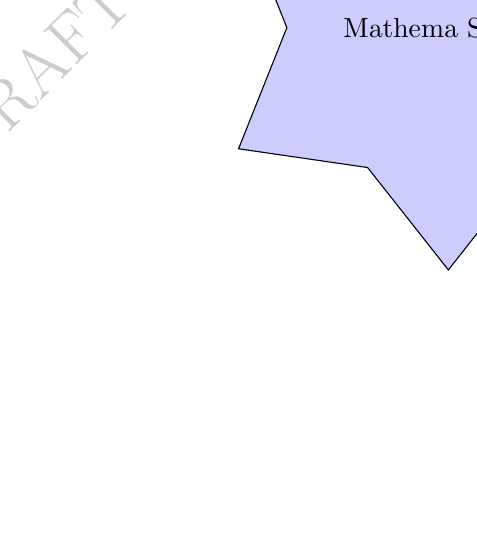
\begin{tikzpicture}
		\tikz \node [fill=blue!20,star,star points=6,draw] {Mathema Shukur };
	\end{tikzpicture}
	\\
	যাদের জন্যে প্রযোজ্যঃ  	\textcolor{magenta}{একাদশ ও দ্বাদশ শ্রেণীর শিক্ষার্থী} \\
	বিষয়ঃ \textcolor{magenta}{উচ্চতর গণিত ১ম পত্র} \\
	অধ্যায়ঃ \textcolor{magenta}{৩-সরলরেখা}\\ 
	Subtopicঃ  \textcolor{magenta}{ ত্রিভুজের ভরকেন্দ্র নির্ণয় করা Centroid of a Triangle }\\
	\\
	ত্রিভুজের যেকোনো দুইটি শীর্ষ বিন্দুর সংযোজক রেখাংশের মধ্যবিন্দু হতে বিপরীত শীর্ষবিন্দু পর্যন্ত সরলরেখা হলো মধ্যমা \\
	\\ 
 ত্রিভুজের মধ্যমা তিনটির ছেদবিন্দুকে ভরকেন্দ্র বলে।\quad $\textcolor{blue}{m=\left(\frac{x_1+x_2+x_3}{3},\frac{y_1+y_2+y_3}{3}\right)}$ \\ 
	\\ 
		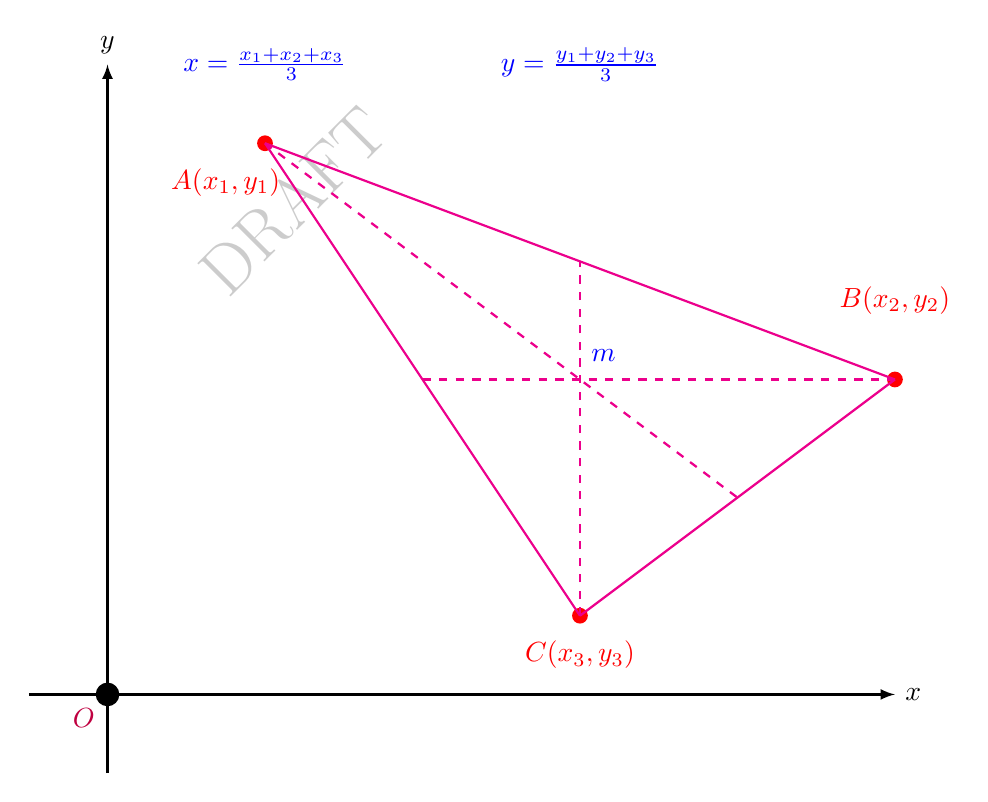
\begin{tikzpicture}[transform shape,scale=1]
		\draw [-latex,thick](-1,0) -- (10,0) node[right] {$x$} coordinate(x axis);
		\draw [-latex,thick](0,-1) -- (0,8) node[above] {$y$} coordinate(y axis);
		\fill[black] (0,0) circle (1.5 mm);
		\node at (-0.3,-0.3) {$\textcolor{purple}{O}$};	
		\fill[red] (2,7) circle (1 mm);
		\fill[red] (6,1) circle (1 mm);
		\fill[red] (10,4) circle (1 mm);
		\node at (6.3,4.3) {$\textcolor{blue}{m}$};
		\node at (1.5,6.5) {$\textcolor{red}{A(x_1,y_1)}$};	
		\node at (6,0.5) {$\textcolor{red}{C(x_3,y_3)}$};
		\node at (10,5) {$\textcolor{red}{B(x_2,y_2)}$};	
		\node at (2,8) {$\textcolor{blue}{x=\frac{x_1+x_2+x_3}{3}}$};			
		\node at (6,8) {$\textcolor{blue}{y=\frac{y_1+y_2+y_3}{3}}$};				
		\draw[thick,magenta] (2,7)--(6,1);
			\draw[thick,magenta,dashed] (2,7)--(8,2.5);
		\draw[thick,magenta] (6,1)--(10,4);
			\draw[thick,magenta,dashed] (6,1)--(6,5.5);
		\draw[thick,magenta] (2,7)--(10,4);
			\draw[thick,magenta,dashed] (4,4)--(10,4);
	\end{tikzpicture}
\\
	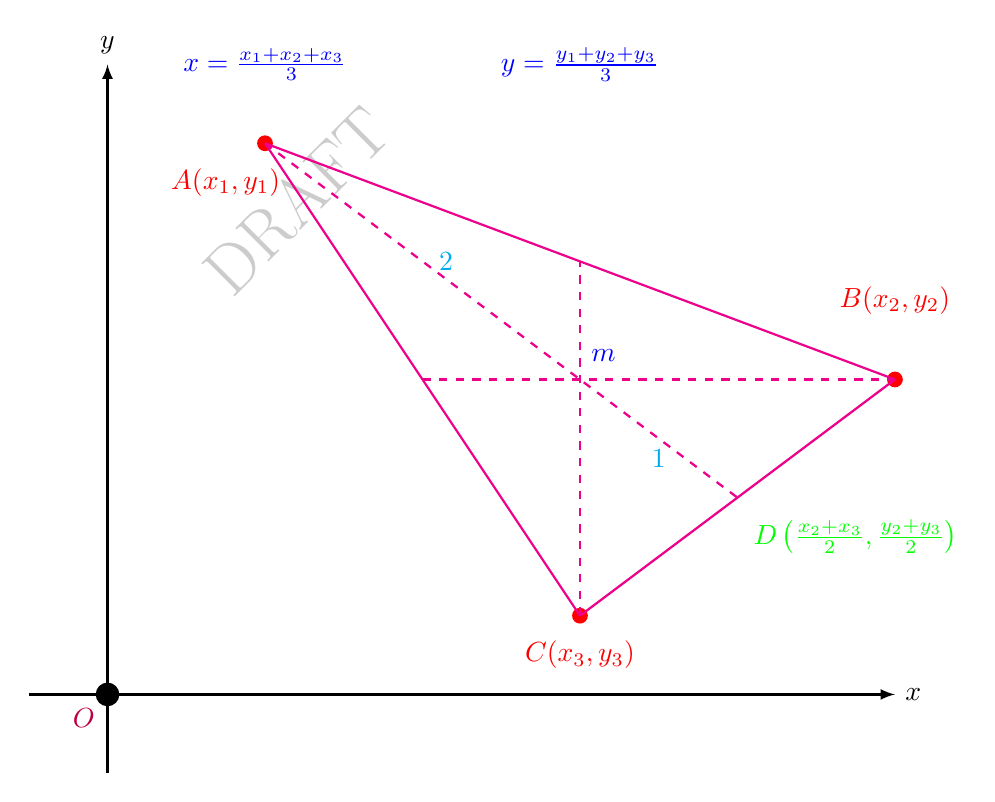
\begin{tikzpicture}[transform shape,scale=1]
	\draw [-latex,thick](-1,0) -- (10,0) node[right] {$x$} coordinate(x axis);
	\draw [-latex,thick](0,-1) -- (0,8) node[above] {$y$} coordinate(y axis);
	\fill[black] (0,0) circle (1.5 mm);
	\node at (-0.3,-0.3) {$\textcolor{purple}{O}$};	
	\fill[red] (2,7) circle (1 mm);
	\fill[red] (6,1) circle (1 mm);
	\fill[red] (10,4) circle (1 mm);
	\node at (9.5,2) {$\textcolor{green}{D\left(\frac{x_2+x_3}{2},\frac{y_2+y_3}{2}\right)}$};
	\node at (6.3,4.3) {$\textcolor{blue}{m}$};
		\node at (4.3,5.5) {$\textcolor{cyan}{2}$};
		\node at (7,3) {$\textcolor{cyan}{1}$};
	\node at (1.5,6.5) {$\textcolor{red}{A(x_1,y_1)}$};	
	\node at (6,0.5) {$\textcolor{red}{C(x_3,y_3)}$};
	\node at (10,5) {$\textcolor{red}{B(x_2,y_2)}$};	
	\node at (2,8) {$\textcolor{blue}{x=\frac{x_1+x_2+x_3}{3}}$};			
	\node at (6,8) {$\textcolor{blue}{y=\frac{y_1+y_2+y_3}{3}}$};				
	\draw[thick,magenta] (2,7)--(6,1);
	\draw[thick,magenta,dashed] (2,7)--(8,2.5);
	\draw[thick,magenta] (6,1)--(10,4);
	\draw[thick,magenta,dashed] (6,1)--(6,5.5);
	\draw[thick,magenta] (2,7)--(10,4);
	\draw[thick,magenta,dashed] (4,4)--(10,4);
\end{tikzpicture}
\begin{multicols}{2}
	$m$ বিন্দুটি  $AD$ রেখাকে $2:1$ অনুপাতে অন্তর্বিভক্ত করে\\  
\begin{align*}
	x&=\frac{2\left(\frac{x_2+x_3}{2}\right)+1\,(x_1)}{2+1}\\
	\\
	x&=\frac{x_1+x_2+x_3}{3}
\end{align*}
\\
\begin{align*}
	y&=\frac{2\left(\frac{y_2+y_3}{2}\right)+1\,(y_1)}{2+1}\\
	\\
	y&=\frac{y_1+y_2+y_3}{3}
\end{align*}
\end{multicols}
	দিনাজপুর বোর্ড-২০১৯\\
	$ABC$ ত্রিভুজের শীর্ষ বিন্দুগুলো $A(2,0)$, $B(5,0)$ ও $C(5,4)$ হলে, ত্রিভুজটির ভরকেন্দ্র নির্ণয় কর । \\ 
	\\ 
	\begin{tikzpicture}[transform shape,scale=1]
		\draw [-latex,thick](-2,0) -- (8,0) node[right] {$x$} coordinate(x axis);
		\draw [-latex,thick](0,-2) -- (0,6) node[above] {$y$} coordinate(y axis);
		\fill[black] (0,0) circle (1.5 mm);
		\node at (-0.3,-0.3) {$\textcolor{purple}{O}$};	
		\fill[red] (2,0) circle (1 mm);
		\fill[red] (5,0) circle (1 mm);
		\fill[red] (5,4) circle (1 mm);
		\node at (4.5,1.2) {$\textcolor{blue}{m}$};
		\node at (1.5,-0.5) {$\textcolor{red}{A(2,0)}$};	
		\node at (5,-0.5) {$\textcolor{red}{B(5,0)}$};
		\node at (5,4.5) {$\textcolor{red}{C(5,4)}$};				
		\draw[thick,magenta] (2,0)--(5,0);
			\draw[thick,magenta,dashed] (2,0)--(5,2);
		\draw[thick,magenta] (5,0)--(5,4);
			\draw[thick,magenta,dashed] (5,0)--(3.5,2);
		\draw[thick,magenta] (2,0)--(5,4);
		\draw[thick,magenta,dashed] (3.5,0)--(5,4);
	\end{tikzpicture}
\\
$(x_1,y_1)=(2,0)$, \quad $(x_2,y_2)=(5,0)$,\quad $(x_3,y_3)=(5,4)$\\
\begin{multicols}{2}
	\begin{align*}
		x&=\frac{x_1+x_2+x_3}{3}\\
		\\
			x&=\frac{2+5+5}{3}\\
			\\
			x&=\frac{12}{3}\\
			\\
			x&=4
	\end{align*}
	\\
	\begin{align*}
		y&=\frac{y_1+y_2+y_3}{3}\\
		\\
		y&=\frac{0+0+4}{3}\\
		\\
		y&=\frac{4}{3}
	\end{align*}
\end{multicols}
ভরকেন্দ্র $(x,y)=(4,\frac{4}{3})$\\
\\
	বরিশাল বোর্ড-২০২১\\
	একটি ত্রিভুজের দুইটি কৌণিক বিন্দুর স্থানাঙ্ক $(-3,4)$ এবং $(5,2)$ । এর ভর কেন্দ্রের স্থানাঙ্ক $(1,4)$ হলে তৃতীয় কৌণিক বিন্দুর স্থানাঙ্ক নির্ণয় কর \\ 
	\\
		\begin{tikzpicture}[transform shape,scale=1]
		\draw [-latex,thick](-4,0) -- (8,0) node[right] {$x$} coordinate(x axis);
		\draw [-latex,thick](0,-2) -- (0,8) node[above] {$y$} coordinate(y axis);
		\fill[black] (0,0) circle (1.5 mm);
		\node at (-0.3,-0.3) {$\textcolor{purple}{O}$};	
		\fill[red] (-3,4) circle (1 mm);
		\fill[red] (5,2) circle (1 mm);
		\fill[red] (1,6) circle (1 mm);
		\node at (1.5,4.3) {$\textcolor{blue}{(1,4)}$};
		\node at (1.5,6.5) {$\textcolor{red}{(a,b)}$};	
		\node at (6,1.5) {$\textcolor{red}{(5,2)}$};
		\node at (-4,4) {$\textcolor{red}{(-3,4)}$};			
		\draw[thick,magenta] (-3,4)--(5,2);
		\draw[thick,magenta] (5,2)--(1,6);
		\draw[thick,magenta] (-3,4)--(1,6);
		\draw[thick,magenta,dashed] (1,3)--(1,6);
		\draw[thick,magenta,dashed] (-1,5)--(5,2);
		\draw[thick,magenta,dashed] (-3,4)--(3,4);
	\end{tikzpicture}
\vspace{6cm}
\\
$(x_1,y_1)=(-3,4)$, \quad $(x_2,y_2)=(5,2)$,\quad $(x_3,y_3)=(a,b)$,\quad $(x,y)=(1,4)$\\
	\begin{multicols}{2}
		\begin{align*}
			x&=\frac{x_1+x_2+x_3}{3}\\
			\\
			1&=\frac{-3+5+a}{3}\\
			\\
			a+2&=3\\
			\\
			a&=1
		\end{align*}
		\\
		\begin{align*}
			y&=\frac{y_1+y_2+y_3}{3}\\
			\\
			4&=\frac{4+2+b}{3}\\
			\\
			b+6&=12\\
			\\
			b&=12-6\\
			\\
			b&=6
		\end{align*}
	\end{multicols}
তৃতীয় কৌণিক বিন্দুর স্থানাঙ্ক $(a,b)=(1,6)$
\end{document}